\documentclass[conference]{IEEEtran}
\IEEEoverridecommandlockouts
% The preceding line is only needed to identify funding in the first footnote. If that is unneeded, please comment it out.
\usepackage{cite}
\usepackage{amsmath,amssymb,amsfonts}
\usepackage{algorithmic}
\usepackage{graphicx}
\usepackage{textcomp}
\usepackage{xcolor}
\usepackage{listings}
\usepackage{tikz}
\usetikzlibrary{arrows.meta, positioning}
\usetikzlibrary{arrows.meta, positioning, shapes.geometric, calc}
\def\BibTeX{{\rm B\kern-.05em{\sc i\kern-.025em b}\kern-.08em
    T\kern-.1667em\lower.7ex\hbox{E}\kern-.125emX}}
\begin{document}

\lstset{
    basicstyle=\ttfamily\footnotesize, % smaller typewriter font
    columns=flexible,
    breaklines=true,
    frame=single,
    backgroundcolor=\color{gray!10}, % light gray background
    tabsize=3, % adjust tab size
    captionpos=b, % sets the caption-position to bottom
}
 
\title{Extending Q-Learning Agents in SQLi Environments}

\author{
    \IEEEauthorblockN{Ryan Marinelli}
    \IEEEauthorblockA{\textit{Department of Informatics} \\
    \textit{University of Oslo}\\
    Oslo, Norway \\
    ryanma@ifi.uio.no}
    \and
    \IEEEauthorblockN{Laszlo Erdődi}
    \IEEEauthorblockA{\textit{Department of Informatics} \\
    \textit{University of Oslo}\\
    Oslo, Norway \\
    laszloe@ifi.uio.no}
}


\maketitle

\begin{abstract}
Q-Learning is one of the foundational techniques in reinforcement learning and provides a benchmark of comparison for other techniques. Reinforcement learning has been used in a plethora of fields and is being increasingly used in Cyber Security. It is being used to automate penetration testing and to perform reconnaissance on vulnerabilities.  The prototypical vulnerability being SQL injection. Previous research efforts have focused on creating agents to exploit these vulnerabilities, but how agents should interact with these environments is still being understood. In this research endeavor, extensions to previous agents using the standard methodology of reinforcement will be extended to measure their effectiveness in a complex environment. Hyper parameter tuning, double Q-Learning, n-step Q-Learning, and using Upper Confidence Bound exploration will be used to provide guidance regarding developing future agents. It is of great importance to understand how these refinements to Q-Learning may empower the agent without having to resort to more sophisticated methods. Other methods may require additional trade-offs and may introduce unfavorable dynamics to the environment. By understanding Q-Learning and related methods, it may be possible to avoid using black box algorithms that would be detrimental to interpretability while still increasing performance.  
\end{abstract}

\begin{IEEEkeywords}
Reinforcement Learning, SQL Injection, Penetration Testing 
\end{IEEEkeywords}

\section{Introduction}
SQL Injection is a vulnerability that continues to persist as an exploit that may be continually found in the wild. Injection vulnerabilities have consistently been listed in the OWSAP top 10 with SQL Injection being a major threat [1]. SQL Injection occurs when a payload is inserted into an application. This is usually done through a field or form meant to interact with the backend. This payload is a query that is meant to probe for information in the application or to manipulate the database.It poses a significant threat to data integrity and needs to be  addressed. 

Reinforcement Learning is a branch of machine learning. The underlying goal is to design an agent that receives a reward and learns a strategy to interact with its environment guided by a specified reward structure. It is rather similar to Pavlov’s dogs in learning a desirable behavior. Through applying reinforcement learning to SQL Injection, it is possible to teach an agent how to inject queries to exploit vulnerable applications. This process is achieved through developing a Markov Decision Process which applies gamification via a reward system. The hope is the agent is able to learn how to identify vulnerable applications, is able to form syntactically correct queries, and exploit the application with the queries. 
\vspace{1mm} % 

The goal of this research is to extend Erdődi et al in which an agent learned to exploit a database through using Q-Learning and Deep Q-Learning Networks. The proposed extension to the work is to consider alternative methodology in their environment to observe how theoretical enhancements would function in their environment. There are several improvements to their agent that will be evaluated. The first is hyper-parameter tuning. Parameters in this context are values used in the learning process. For instance, gamma is typically used as a temporal discount factor. You may want the agent to consider actions in the future more or less based on your expectations of how it will interact. In the previous paper, this does not seem to develop in a principled manner but more so on the experience of the authors. By iterating through a search of values, it is possible to determine more optimal values than those informed on experience alone. Additionally, Upper Confidence Bound will be used to guide the agent in exploration. Agents must often choose between attempting a new task to see if they will get more reward or to do the reward that is already known to be most beneficial. This is the exploration vs exploitation trade-off that must be balanced. In Erodi et al, the method to navigate this is epsilon-greedy: an epsilon amount of time the agent will choose to explore. With UCB, a confidence interval to make the determination is often more performant. Outside of these general methodological advancements, there are more sophisticated extensions from Q-Learning. Double-Q Learning and N-Step Q-Learning will be applied as they are natural extensions to the base Q-Learning agent. Through applying these advancements with agents and methodology, perhaps the Q-Learning agent may be more performant than using deep learning. This would be a significant gain given that deep learning models are rather difficult to interpret and Q-Learning allows for a more understandable transition of the agent. 

\section{Algorithms}
\vspace{-3mm}
Due to the nature of this endeavour, it will be useful to discuss the foundational algorithms used in reinforcement learning, within Erdődi et al, and those used as an extension. It should be useful to create the comparisons between methods and to see more clearly which methods are being extended more specifically. 

\subsection{Update Rules}
Update rules are the methods that agents use to learn. They provide guidance with how far the agent should look into the future or how it should weigh actions and optimize reward. 

\vspace{2mm}
\paragraph{Bellman Equation}
The Bellman Equation is central to Q-Learning. It expresses the relationship with states and actions with successor states. It is this recursive relationship that allows it to be used as an update rule to find optimal values. States can be understood where the agent is at. It is a composition of a chessboard at a particular time. An action is the next move the agent should do. The states reached by the agent and the actions selected are selected based on maximizing cumulative reward, $R(s,a)$. $\gamma$ is a temporal discount factor.  $P(s' \mid s, a)$ describes the probability of transitioning to different states. It provides dynamics to the equation.  

\vspace{-4mm}
\begin{equation}
    Q^*(s, a) = R(s, a) + \gamma \sum_{s'} P(s' \mid s, a) \max_{a'} Q^*(s', a') 
\end{equation}

\vspace{-2mm}
\paragraph{Q-Learning}
Q-Learning applies the Bellman Equation as an update rule to a table. This Q-table is a matrix storing Q values for each state-action pair. When an agent performs an action, the new reward gets observed, and a new state is reached. Then, the Bellman Equation updates the table in an iterative fashion. 
\begin{equation}
    Q^{new}(s, a) = Q(s, a) + \alpha \left[ r + \gamma \max_{a'} Q(s', a') - Q(s, a) \right]
\end{equation}

\paragraph{Double Q-Learning}
Double Q-Learning aims to address the overestimation bias found in Q-Learn. In Q-Learning, the maximization step may introduce error. When an agent is starting to learn, the Q-values are substantially more noisy, and a sub-optimal may be selected. This may change the trajectory adding bias that will not be corrected. 

By adding a second Q-table and choosing values with equal probability, then this bias may be reduced.

\begin{equation}
\begin{split}
    &\text{With probability 0.5:} \\
    &Q_A(s, a) \leftarrow Q_A(s, a) + \\
    &\quad \alpha \big[ r + \gamma Q_B\left(s', \max_{a'} Q_A(s', a')\right) - Q_A(s, a) \big], \\
    &\text{Otherwise:} \\
    &Q_B(s, a) \leftarrow Q_B(s, a) + \\
    &\quad \alpha \big[ r + \gamma Q_A\left(s', \max_{a'} Q_B(s', a')\right) - Q_B(s, a) \big].
\end{split}
\end{equation}

\paragraph{N-Step Q-Learning}
N-Step Q-Learns uses more than the next step to update Q-values which is what occurs in traditional Q-Learning. It bases Q-values on N next steps. It essentially estimates the aggregated expected future rewards that is discounted by $\gamma$.  
\begin{equation}
\begin{aligned}
Q(S_t, A_t) & \leftarrow Q(S_t, A_t) + \alpha \Bigg( \sum_{k=0}^{n-1} \gamma^k R_{t+k+1} \\
            & \quad + \gamma^n \max_a Q(S_{t+n}, a) - Q(S_t, A_t) \Bigg)
\end{aligned}
\end{equation}

This approach is more suited for coping with delayed rewards. Given the complex nature of attempting to figure out the payload, this may yield better results. It also gives more control concerning when to update. Some update rules wait until the end to update, but the update might be significant for the agent to learn. Other methods update online with each step. In this instance, agents might be overly responsive to variance. By selecting amount of steps to consider, it strikes more of a balancing act that should lead to more stable rewards.  

\subsection{Exploration Strategies}
Exploration strategies are deployed by agents to help them navigate the exploration-exploitation trade-off. 

\paragraph{Epsilon-Greedy}
With $\epsilon$ greedy strategies, the agent chooses a random action  $\epsilon$ amount of the time. This is to encourage the agent to explore and not select a sub-optimal action. 
\[
A_t = 
\begin{cases} 
\text{random action} & \text{with probability } \epsilon, \\
\arg\max_a Q_t(a) & \text{with probability } 1 - \epsilon,
\end{cases}
\]
\paragraph{Upper Confidence Bound}

This exploration method uses the average reward of an action at time $t$ and uses the confidence interval term,  $\sqrt{\frac{2 \ln t}{N_a(t)}}$, to determine the bounds. 
\[
\text{UCB}(a, t) = \bar{X}_a(t) + \sqrt{\frac{2 \ln t}{N_a(t)}}
\]

The action with the values located with the upper most bounds is selected. By using a logarithmic term, the amount of exploration slows providing a smoothing effect allowing the exploration to balance exploration with exploitation. 

\paragraph{Hyperparameter Tuning}
Hyperparameter selection is a factoring determining how to best optimize the behavior of agents. In this case, $\gamma$, a discount factor, $\alpha$, the learning rate, $\epsilon$, the exploration rate, and max numbers of steps are determined through applying Bayesian techniques 

\paragraph{ Tree-structured Parzen Estimation}
TPE is an approach to modeling the distributions of the hyperparmeters.It follows several stages: a sampling stage to form a prior, an update of the Probability Density functions $l(x)$ and $g(x)$, and maximizing Expected Improvement $EI$.

\[
\text{EI}(x) = \frac{l(x)}{g(x)}
\]
$l(x)$ represents effectively well a specific configuration of hyperparameters performed based on an objective function provided. In this case, it is optimizing for the inverse reward  as `Optuna`, the Python library used to perform this, treats it as a minimization problem. $g(x)$ is the density function where a configure performed poorly as defined by the objective function and a specific $y*$, a point on the distribution to classify how to update the density functions. The optimal values determined through this method through sampling where $l(x)$ is high and $g(x)$ is low

\section{SQL Injection}
SQL injection is a vulnerability that occurs through the improper validation of user-input in the backend of an application. SQL queries are submitted as a payload to manipulate the database or access underlying data. It requires expertise to probe the application due to the nature of SQL syntax. An attack must infer which variety of SQL is being deployed on the server during their reconnaissance. There are various varieties of SQL injection attack methods, but the two explored in Erdődi et al are based on using UNION joins and boolean conditions. Of the of the common Boolean conditions is to use "1=1" with the matching escape characters. If the boolean condition is true, the OR clause will return data from the attack target. BURP is a popular tool in conducting attacks, and deploys an interface for interacting with the out-going HTTP requests to the target.

\begin{figure}[ht]
\begin{lstlisting}
POST /login HTTP/1.1
Host: target.com
Content-Type: application/x-www-form-urlencoded
Content-Length: length

username=admin' OR '1'='1&password=admin' OR '1'='1

\end{lstlisting}
\caption{SQL injection using Boolean Conditions}
\label{fig:booleanrequest}
\end{figure}

As for UNION attacks, one can use the operator to pull data from other target tables. The request to recover username and password might look like Fig 2. 

\begin{figure}[ht]
\begin{lstlisting}
POST /login HTTP/1.1
Host: target.com
Content-Type: application/x-www-form-urlencoded
Content-Length: 180

username=admin' UNION SELECT username, password FROM users-- &password=

\end{lstlisting}
\caption{SQL injection with UNION}
\label{fig:unionrequest}
\end{figure}

\noindent The general pattern described by Erd\H{o}di et al. to conduct SQL Injection is outlined as follows:

\begin{enumerate}
  \item \textbf{Find a Vulnerable Input Parameter:} Identify parameters that are improperly validated. In the discussed example, the vulnerable parameters are \textit{username} and \textit{password}.

  \item \textbf{Detect the Type of Vulnerable Input Parameter:} The attacker needs to understand how queries are being processed in the backend of the application. Proper formatting of escape characters is crucial. In the examples given, the single quote is used to escape, allowing the attacker to insert their payload.

  \item \textbf{Continue the SQL Query Without Syntax Errors:} The payload defined by the attacker must conform to the expected SQL syntax and adapt to different SQL types (e.g., PostgreSQL, MySQL) while properly escaping characters.

  \item \textbf{Obtain the SQL Answer Presentation in the HTTP Response:} By submitting requests and observing the response, the attacker can infer characteristics about the database. Notable observations may include differences in the HTML response or HTTP behavior, which inform further payloads.

  \item \textbf{Obtain Database Characteristics for More Advanced Queries:} With an understanding of the database, the attacker can craft more precise queries to explore the database structure, including tables and their contents.

  \item \textbf{Obtain Sensitive Information:} The attacker formulates queries using boolean conditions or UNION operations to extract information of interest.

  \item \textbf{Carry Out Extra Operation:} The attacker may attempt to disrupt operations by executing commands to DROP tables, rendering the database unusable.
\end{enumerate}

\section{The Environment}
A Markov Decision Process is a framework for modeling Reinforcement agents. As largely described during the discussion of the  Bellman Equation, there are states, actions, transition functions, reward functions, and discount factors. The agent selects actions based on the reward and enters different states based on transition probability. The components of the MDP mutally interact to describe the dynamics of a particular system.

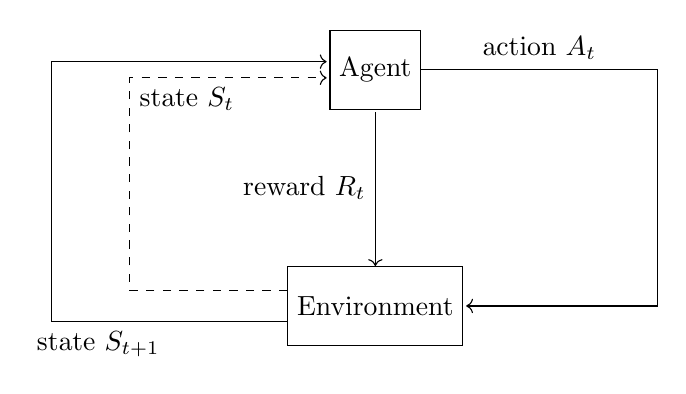
\begin{tikzpicture}[shorten >=1pt,auto,node distance=3cm]
    \node[rectangle, draw, minimum size=1cm] (agent) {Agent};
    \node[rectangle, draw, below of=agent, minimum size=1cm] (environment) {Environment};

    \draw[->] (agent.0) -- node {action $A_t$} ++(3cm,0) |- (environment.0);
    \draw[->] (environment.190) -- node[below left] {state $S_{t+1}$} ++(-3cm,0) |- (agent.170);
    \draw[<-] (environment) -- node {reward $R_{t}$} (agent);

    \draw[->,dashed] (environment.170) -- ++(-2cm,0) |- node[below right] {state $S_t$} (agent.190);

\end{tikzpicture}


\subsection{Model}
In L. Erdődi et al, the complexity of SQL Injection was refined into a model to fit into an MDP formulation. One of the main points is the adoption of a Capture-The-Flag formulation. Often in cyber security settings, a flag, usually a string or hash, is hidden for the attack in training to find. By using this game like setting, Erdődi was able to define the environment. Additional constraints were imposed as well. In the environment, there should only be one vulnerable parameter, no input validation by the server side script. UNION will be allowed to match with columns, and that error messages will not be accessible by the attacker. 

Within the consideration of the MDP, the set of states maps to the server. Since the web server in Erdődi et al is stateless; it is a singleton state. A reward function is used to guide agent. A +10 reward is awarded for finding the flag and a -1 reward is used as a disincentive. The action space is defined by attempting to determine the escape character and finding the columns to insert into for injection. The state space is defined by the action space. 

\subsection{Identify the Headings}
Headings, or heads, are organizational devices that guide the reader through 
your paper. There are two types: component heads and text heads.

Component heads identify the different components of your paper and are not 
topically subordinate to each other. Examples include Acknowledgments and 
References and, for these, the correct style to use is ``Heading 5''. Use 
``figure caption'' for your Figure captions, and ``table head'' for your 
table title. Run-in heads, such as ``Abstract'', will require you to apply a 
style (in this case, italic) in addition to the style provided by the drop 
down menu to differentiate the head from the text.

Text heads organize the topics on a relational, hierarchical basis. For 
example, the paper title is the primary text head because all subsequent 
material relates and elaborates on this one topic. If there are two or more 
sub-topics, the next level head (uppercase Roman numerals) should be used 
and, conversely, if there are not at least two sub-topics, then no subheads 
should be introduced.

\subsection{Figures and Tables}
\paragraph{Positioning Figures and Tables} Place figures and tables at the top and 
bottom of columns. Avoid placing them in the middle of columns. Large 
figures and tables may span across both columns. Figure captions should be 
below the figures; table heads should appear above the tables. Insert 
figures and tables after they are cited in the text. Use the abbreviation 
``Fig.~\ref{fig}'', even at the beginning of a sentence.

\begin{table}[htbp]
\caption{Table Type Styles}
\begin{center}
\begin{tabular}{|c|c|c|c|}
\hline
\textbf{Table}&\multicolumn{3}{|c|}{\textbf{Table Column Head}} \\
\cline{2-4} 
\textbf{Head} & \textbf{\textit{Table column subhead}}& \textbf{\textit{Subhead}}& \textbf{\textit{Subhead}} \\
\hline
copy& More table copy$^{\mathrm{a}}$& &  \\
\hline
\multicolumn{4}{l}{$^{\mathrm{a}}$Sample of a Table footnote.}
\end{tabular}
\label{tab1}
\end{center}
\end{table}

\begin{figure}[htbp]
\centerline{\includegraphics{fig1.png}}
\caption{Example of a figure caption.}
\label{fig}
\end{figure}

Figure Labels: Use 8 point Times New Roman for Figure labels. Use words 
rather than symbols or abbreviations when writing Figure axis labels to 
avoid confusing the reader. As an example, write the quantity 
``Magnetization'', or ``Magnetization, M'', not just ``M''. If including 
units in the label, present them within parentheses. Do not label axes only 
with units. In the example, write ``Magnetization (A/m)'' or ``Magnetization 
\{A[m(1)]\}'', not just ``A/m''. Do not label axes with a ratio of 
quantities and units. For example, write ``Temperature (K)'', not 
``Temperature/K''.

\section*{Acknowledgment}

The preferred spelling of the word ``acknowledgment'' in America is without 
an ``e'' after the ``g''. Avoid the stilted expression ``one of us (R. B. 
G.) thanks $\ldots$''. Instead, try ``R. B. G. thanks$\ldots$''. Put sponsor 
acknowledgments in the unnumbered footnote on the first page.

\section*{References}

Please number citations consecutively within brackets \cite{b1}. The 
sentence punctuation follows the bracket \cite{b2}. Refer simply to the reference 
number, as in \cite{b3}---do not use ``Ref. \cite{b3}'' or ``reference \cite{b3}'' except at 
the beginning of a sentence: ``Reference \cite{b3} was the first $\ldots$''

Number footnotes separately in superscripts. Place the actual footnote at 
the bottom of the column in which it was cited. Do not put footnotes in the 
abstract or reference list. Use letters for table footnotes.

Unless there are six authors or more give all authors' names; do not use 
``et al.''. Papers that have not been published, even if they have been 
submitted for publication, should be cited as ``unpublished'' \cite{b4}. Papers 
that have been accepted for publication should be cited as ``in press'' \cite{b5}. 
Capitalize only the first word in a paper title, except for proper nouns and 
element symbols.

For papers published in translation journals, please give the English 
citation first, followed by the original foreign-language citation \cite{b6}.

\begin{thebibliography}{00}
\bibitem{b1} G. Eason, B. Noble, and I. N. Sneddon, ``On certain integrals of Lipschitz-Hankel type involving products of Bessel functions,'' Phil. Trans. Roy. Soc. London, vol. A247, pp. 529--551, April 1955.
\bibitem{b2} J. Clerk Maxwell, A Treatise on Electricity and Magnetism, 3rd ed., vol. 2. Oxford: Clarendon, 1892, pp.68--73.
\bibitem{b3} I. S. Jacobs and C. P. Bean, ``Fine particles, thin films and exchange anisotropy,'' in Magnetism, vol. III, G. T. Rado and H. Suhl, Eds. New York: Academic, 1963, pp. 271--350.
\bibitem{b4} K. Elissa, ``Title of paper if known,'' unpublished.
\bibitem{b5} R. Nicole, ``Title of paper with only first word capitalized,'' J. Name Stand. Abbrev., in press.
\bibitem{b6} Y. Yorozu, M. Hirano, K. Oka, and Y. Tagawa, ``Electron spectroscopy studies on magneto-optical media and plastic substrate interface,'' IEEE Transl. J. Magn. Japan, vol. 2, pp. 740--741, August 1987 [Digests 9th Annual Conf. Magnetics Japan, p. 301, 1982].
\bibitem{b7} M. Young, The Technical Writer's Handbook. Mill Valley, CA: University Science, 1989.
\end{thebibliography}
\vspace{12pt}
\color{red}
IEEE conference templates contain guidance text for composing and formatting conference papers. Please ensure that all template text is removed from your conference paper prior to submission to the conference. Failure to remove the template text from your paper may result in your paper not being published.

\end{document}
